\chapter{実験}
予備実験を含め、実験は5種類行なった.

\section{予備実験}
\subsection{動画像平均画像クラス分類}
DCAD,レスキュー犬訓練データセットで分類を行なった.
DCADはクリップ毎にフレーム間の平均をとり,画像として扱ってVGG16のpretrained modelを用いてfinetuningを行なった.
レスキュー犬訓練データセットは動画をラベル毎に切り出して短いクリップ群を作り,そのクリップ毎に同様にフレーム間の平均を取った画像を作成しVGG16のpretrained modelを用いてfinetuningした.

%\section{オプティカルフロー動画平均画像クラス分類}
%動画像のフレーム間の平均を取った手法と同様に,クリップ毎にoptical flowの平均画像を作成しVGG16のpretrained modelを用いてfinetuningを行なった.

\section{動画像からのマルチクラス推定}
\section{オプティカルフロー画像からのマルチクラス推定}
\begin{table}[tb]
 \centering
 \caption{回数}\label{cyberdataset_label}
 \scalebox{1.00}[1.00]{
  \begin{tabular}{|l||c|c|c|c|c|c|c|c|c|c|c|c|}
   \hline \hline
   クラス   & bark& cling&command& eat&handler& run&victim& shake& sniff& stop& walk & 全体\\ \hline
   Precision& & & & & & & & & & & 0.5305\\ \hline
   Recall   & & & & & & & & & & & \\ \hline
   Jaccard  & & & & & & & & & & & \\ \hline
  \end{tabular}
 }

%\begin{figure}[htbp]
% \begin{center}
%  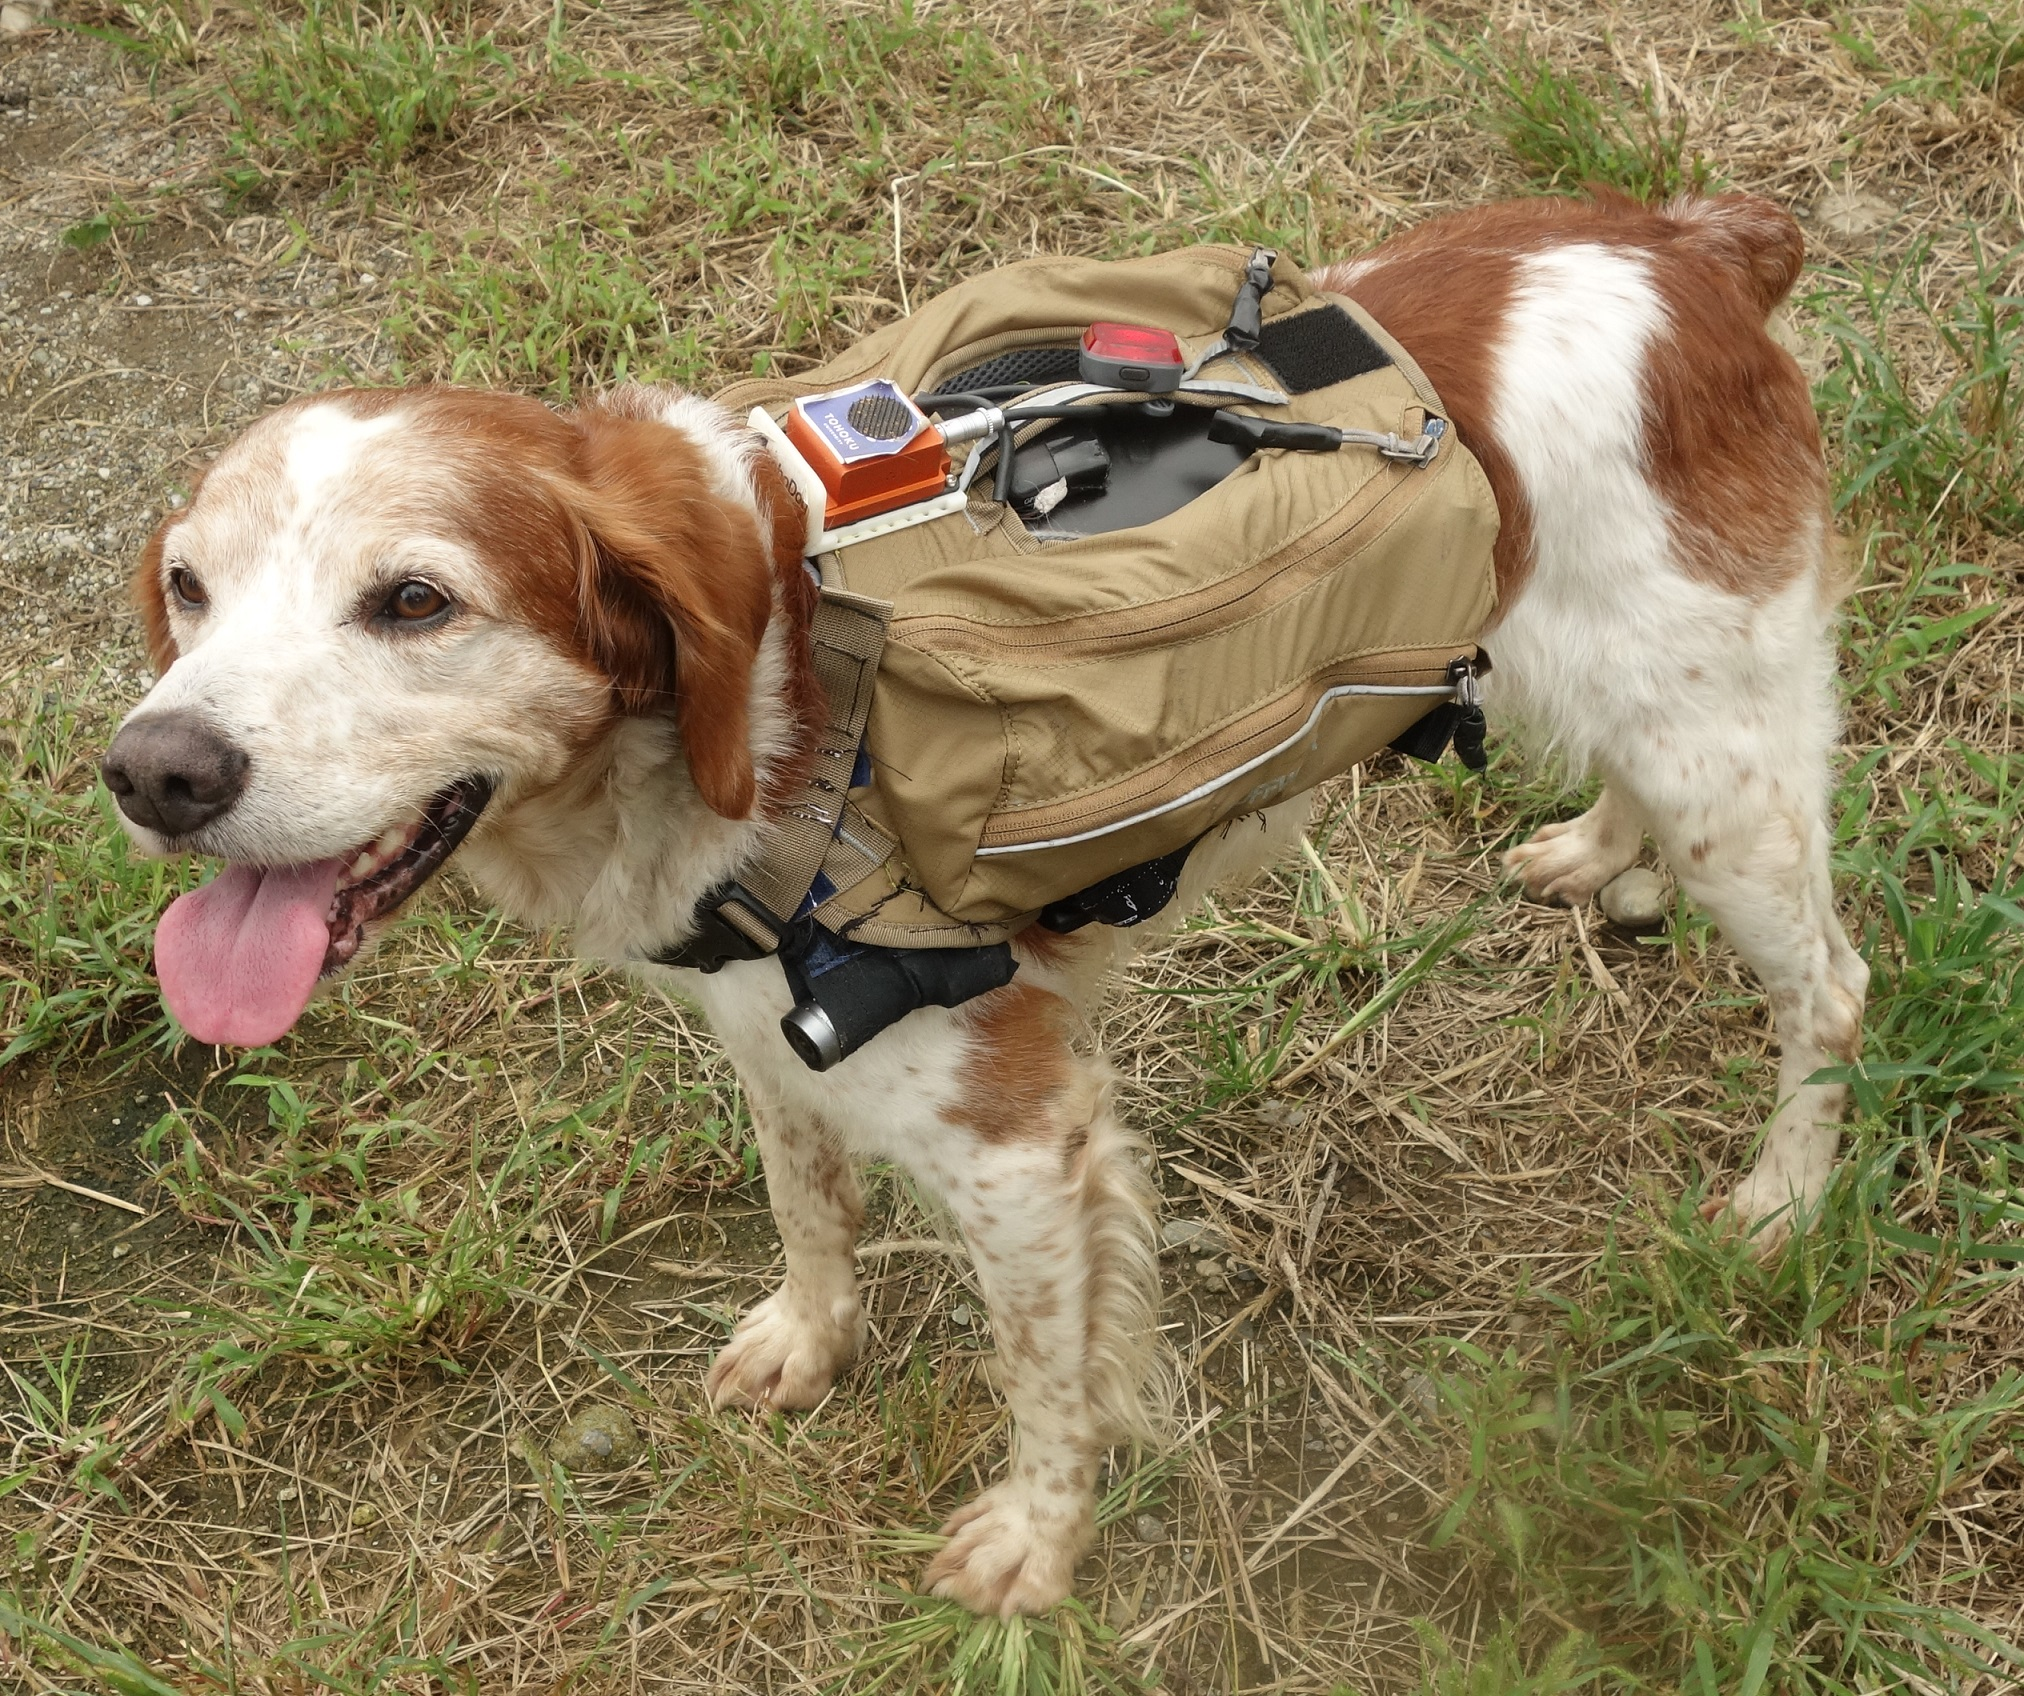
\includegraphics[width=9cm]{./Figures/cyberdog.eps}
%  \caption{装着型計測・記録装置~\cite{dog01}より引用}
%  \label{cyberdog}
% \end{center}
%\end{figure}
\section{音声からのマルチクラス推定}
\section{Two-stream}
\section{Sound based Two-stream}
\section{Sound based Three-stream}
